\documentclass{article}
\usepackage[T1]{fontenc}
\usepackage[utf8]{inputenc}
\usepackage[margin = 1in]{geometry}

\usepackage{amsmath}
\usepackage{amsthm}
\usepackage{amsfonts}
\usepackage{amssymb}
\usepackage{palatino}
\usepackage{tikz-cd}
\usetikzlibrary{automata}
\usepackage{pgfplots}
\pgfplotsset{compat = 1.17}

% https://tex.stackexchange.com/questions/37185/typesetting-a-directed-weighted-graph-with-tikz

\tikzset{
    > = stealth,
    every path/.style = {->, thick}
}

\begin{document}

% maximum-flow/res_2
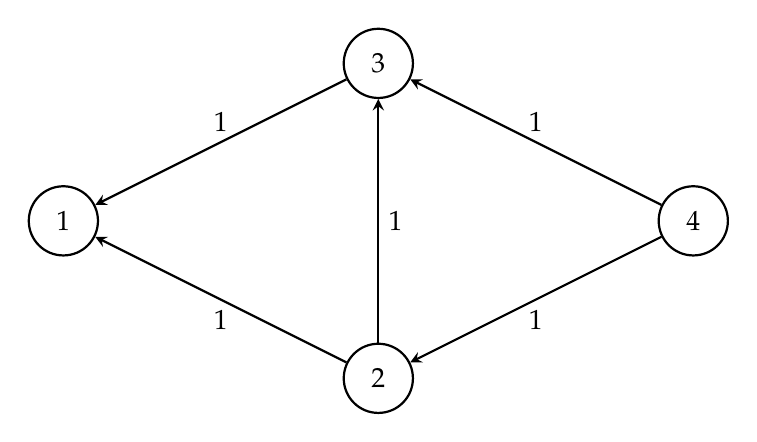
\begin{tikzpicture}
    \node[state] (1) at (0, 2) {1};
    \node[state] (2) at (4, 0) {2};
    \node[state] (3) at (4, 4) {3};
    \node[state] (4) at (8, 2) {4};

    \draw (2) edge node[below]{1} (1);
    \draw (3) edge node[above]{1} (1);
    \draw (2) edge node[right]{1} (3);
    \draw (4) edge node[below]{1} (2);
    \draw (4) edge node[above]{1} (3);
\end{tikzpicture}

\iffalse
% maximum-flow/aug_path_2
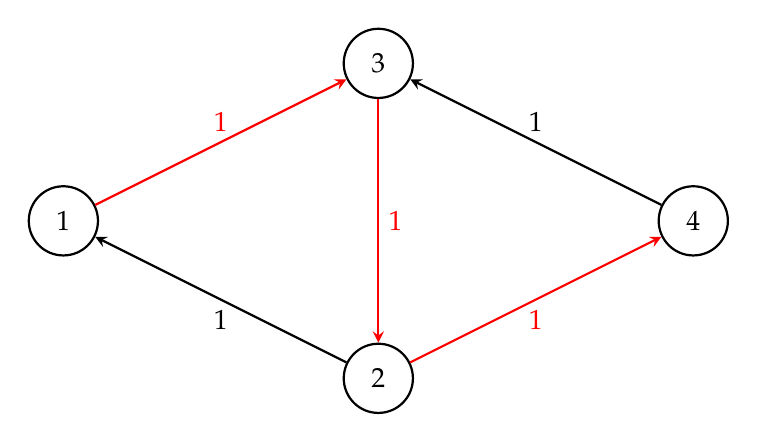
\begin{tikzpicture}
    \node[state] (1) at (0, 2) {1};
    \node[state] (2) at (4, 0) {2};
    \node[state] (3) at (4, 4) {3};
    \node[state] (4) at (8, 2) {4};

    \draw (2) edge node[below]{1} (1);
    \draw (1) edge[red] node[above]{1} (3);
    \draw (3) edge[red] node[right]{1} (2);
    \draw (2) edge[red] node[below]{1} (4);
    \draw (4) edge node[above]{1} (3);
\end{tikzpicture}
\fi

\iffalse
% maximum-flow/res_1
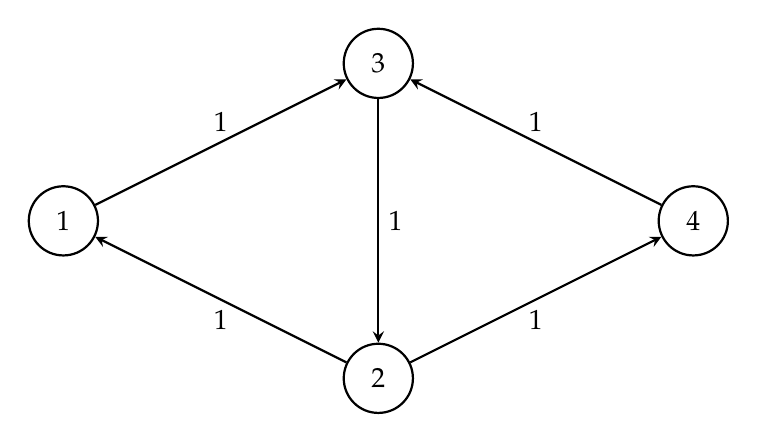
\begin{tikzpicture}
    \node[state] (1) at (0, 2) {1};
    \node[state] (2) at (4, 0) {2};
    \node[state] (3) at (4, 4) {3};
    \node[state] (4) at (8, 2) {4};

    \draw (2) edge node[below]{1} (1);
    \draw (1) edge node[above]{1} (3);
    \draw (3) edge node[right]{1} (2);
    \draw (2) edge node[below]{1} (4);
    \draw (4) edge node[above]{1} (3);
\end{tikzpicture}
\fi

\iffalse
% maximum-flow/flow_1
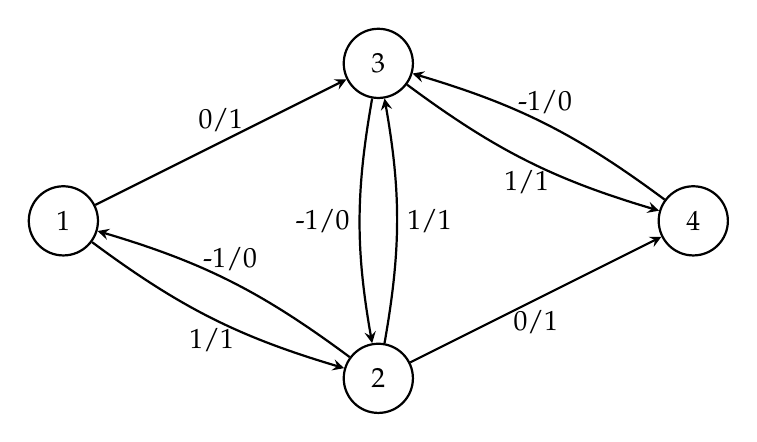
\begin{tikzpicture}
    \node[state] (1) at (0, 2) {1};
    \node[state] (2) at (4, 0) {2};
    \node[state] (3) at (4, 4) {3};
    \node[state] (4) at (8, 2) {4};

    \draw (1) edge[bend right = 10] node[below]{1/1} (2);
    \draw (2) edge[bend right = 10] node[above]{-1/0} (1);
    \draw (1) edge node[above]{0/1} (3);
    \draw (2) edge[bend right = 10] node[right]{1/1} (3);
    \draw (3) edge[bend right = 10] node[left]{-1/0} (2);
    \draw (2) edge node[below]{0/1} (4);
    \draw (3) edge[bend right = 10] node[below]{1/1} (4);
    \draw (4) edge[bend right = 10] node[above]{-1/0} (3);
\end{tikzpicture}
\fi

\iffalse
% maximum-flow/aug_path_1
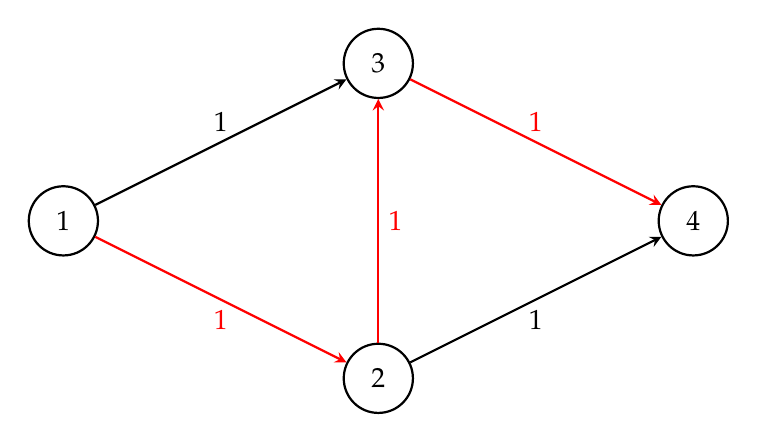
\begin{tikzpicture}
    \node[state] (1) at (0, 2) {1};
    \node[state] (2) at (4, 0) {2};
    \node[state] (3) at (4, 4) {3};
    \node[state] (4) at (8, 2) {4};

    \draw (1) edge[red] node[below]{1} (2);
    \draw (1) edge node[above]{1} (3);
    \draw (2) edge[red] node[right]{1} (3);
    \draw (2) edge node[below]{1} (4);
    \draw (3) edge[red] node[above]{1} (4);
\end{tikzpicture}
\fi

\iffalse
% maximum-flow/flow
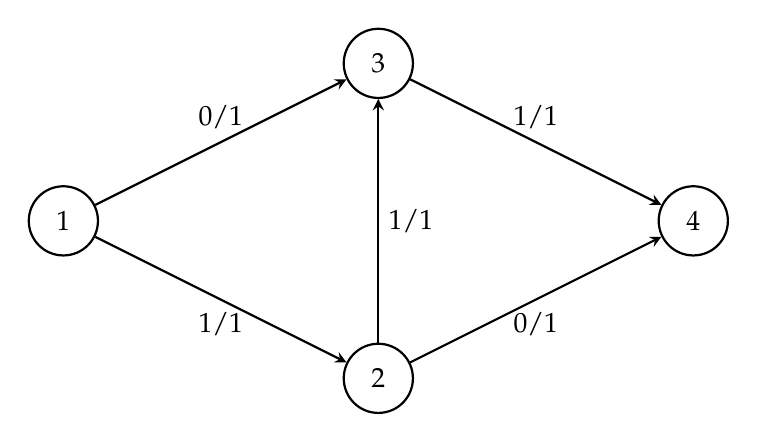
\begin{tikzpicture}
    \node[state] (1) at (0, 2) {1};
    \node[state] (2) at (4, 0) {2};
    \node[state] (3) at (4, 4) {3};
    \node[state] (4) at (8, 2) {4};

    \draw (1) edge node[below, yshift = -1]{1/1} (2);
    \draw (1) edge node[above, yshift = 1]{0/1} (3);
    \draw (2) edge node[right]{1/1} (3);
    \draw (2) edge node[below, yshift = -1]{0/1} (4);
    \draw (3) edge node[above, yshift = 1]{1/1} (4);
\end{tikzpicture}
\fi

\iffalse
% maximum-flow/network
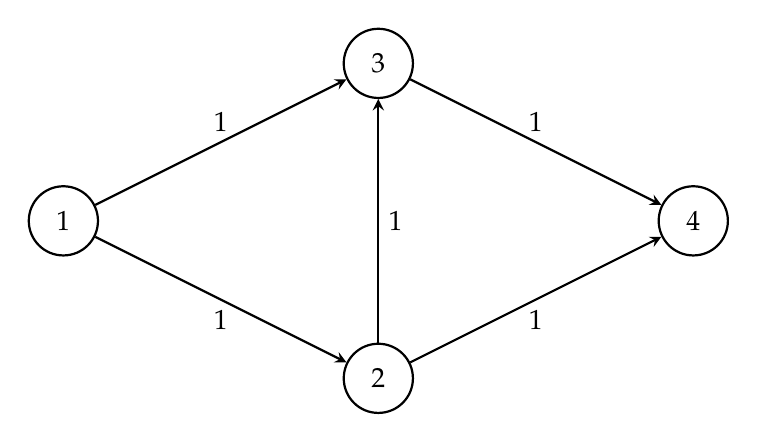
\begin{tikzpicture}
    \node[state] (1) at (0, 2) {1};
    \node[state] (2) at (4, 0) {2};
    \node[state] (3) at (4, 4) {3};
    \node[state] (4) at (8, 2) {4};

    \draw (1) edge node[below]{1} (2);
    \draw (1) edge node[above]{1} (3);
    \draw (2) edge node[right]{1} (3);
    \draw (2) edge node[below]{1} (4);
    \draw (3) edge node[above]{1} (4);
\end{tikzpicture}
\fi

\end{document}
